\documentclass{article}
\usepackage{graphicx} % Required for inserting images
\usepackage[margin=1.0in]{geometry}
\usepackage{float}
\usepackage{hyperref}
\usepackage{listings}



\linespread{1}
\setlength{\parindent}{0pt} % Disable paragraph indentation

\title{Detailed Project Explanation}
\author{Group: G6}
\date{December 6th, 2024}

\begin{document}

\maketitle


\section{Part I}



\subsection{Structure}
The general structure for Part I was already provided. We only needed to complete the methods for the "Game" class, such as the superloop, move, calculateNewCoordinates, isGameOver and is createNewPrey methods.

\subsection{Implementation}

\subsubsection{New Snake Coordinates}
This method is very straightforward. It checks the direction by accessing \texttt{self.direction} to determine which direction the head of the snake should travel, and adding/subtracting the \texttt{SNAKE\_ICON\_WIDTH} by the current x or y coordinate.

\subsubsection{Prey Generation}
To generate the prey, we used the \texttt{random} library to generate a random integer for the x direction and the y direction on the Tkinter canvas. We added a small margin so the prey did not generate on or outside the edges of the window.
\subsubsection{Prey Capture}
One of the primary challenges we faced was implementing the prey capture logic. Since prey can spawn at any location on the Tkinter canvas, iterating through a list of tuples to compare coordinates is both resource-intensive and time-consuming. To optimize this process and eliminate the need for nested "for" loops, we calculated the corner coordinates of both the prey and the snake's head. We then checked whether any point of the snake's head fell within the prey's boundaries, as illustrated in figure \ref{fig:prey_capture}. This method works effectively when the prey is larger than the snake. In cases where the snake is significantly larger than the prey, we reversed the logic: if any point of the prey fell within the snake's boundaries, it would be counted as a collision.
\begin{figure}[H]
   \centering
    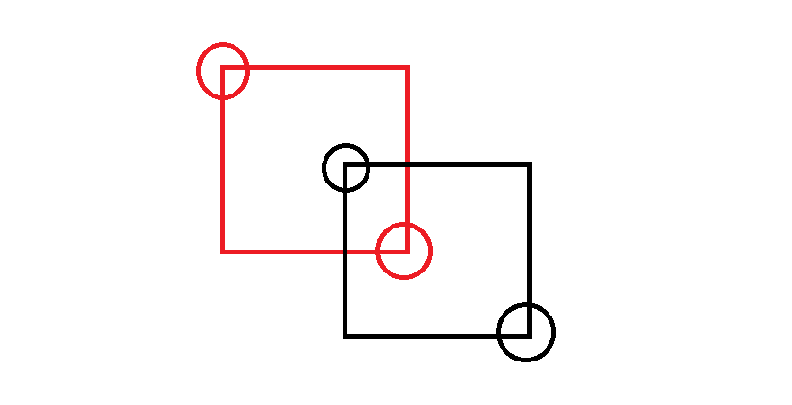
\includegraphics[width=0.6\textwidth]{prey_capture.png}
    \caption{Prey Capture Logic}
    \label{fig:prey_capture}

\end{figure}

This solution mitigates the amount of recursion performed, while still detecting snake and prey collision.
\subsubsection{Move}
This method completes most the important game logic once the snake moves. Firstly, we had to check whether the prey is captured. If true, we added one to the score, increased the length of the snake, and created a new prey. Otherwise, the length of the snake would not change. Checking if the game is over is also necessary. Tasks are added to the queue are added here so the QueueHandler could manage edits to the GUI.
\subsubsection{Game Over Logic}
The game ends once:
\begin{itemize}
    \item the snake's head either goes out of bounds, OR
    \item the snake runs into itself.
\end{itemize}
We checked whether the coordinates of the snake's head are outside the bounds of the Tkinter canvas or if the head coordinate is the same as any of the other snake coordinates.


\section{Part I Alternative}

\subsection{Modified Approach}
For the Part I Alternative, our one main modification to Part I was to remove the use of the QueueHandler class. This was replaced by the GUI class scheduling GUI updates every 100ms using \texttt{self.root.after(100, self.update)}. Since the GUI and move thread are performing operations simultaneously, we had to add locks to ensure data was not being modified as the changes were being updated by the GUI. The GUI processes used non-blocking locks so none of the GUI methods stalled while waiting for the move thread to either read or write the data.

\section{Part II}
\subsection{Structure}

% short description of the Sequence Diagram above
\subsection{Implementation}
This section will only discuss the more complicated chunks of code to maintain conciseness.
\subsubsection{Server}
{\small \textbf{Accepting Clients}} \\
This method is run by a thread which is being infinitely called, constantly checking for new clients or reconnecting clients. In that case, it first \texttt{.accept()}s the client socket and runs each client thread. The client threads are responsible to handle messages for each client.

\

{\small \textbf{Message Handling}} \\
Each of the client threads are responsible for checking for new data. In the case there's an socket error, the thread would be killed. Otherwise it would decode the message sent by the client using \texttt{.decode(MAX\_BYTES)} method and would be sent to the TCP method to send to each of the client sockets.

\

{\small \textbf{Sending TCP}} \\
The TCP is responsible to send messages from one of the clients to all the clients. Although a trivial solution would be to just use the \texttt{.send(MESSAGE)} method to each of the client sockets, this would require excessive use of the mutex lock when accessing the instance variable \texttt{self.socketInfo}, which would prohibit the client threads from operating in parallel, especially if multiple clients are sending messages simultaneously. Instead, we decided to make a copy of the \texttt{self.socketInfo} instance and using \texttt{.send()} for any online clients. In the case that one of the clients goes offline, this socket would be appended to \texttt{staleInfo} list which would remove each stale socket from the \texttt{self.socketInfo} instance. The code is shown in the snippet below.

\begin{lstlisting} [language=Python, label={lst:tcp}, basicstyle=\ttfamily\tiny]
def __send_tcp(self, msg: str) -> None:
        self.lock.acquire() # Critical Section (Start)
        readInfo: list[dict] = self.socketInfo.copy()
        self.lock.release() # Critical Section (End)

        staleInfo: list[dict] = []
        for info in readInfo:
            try:
                info["socket"].send(msg.encode())
            except socket.error:
                staleInfo.append(info) # Remove Info
        self.display_msg(msg)

        for info in staleInfo:
            self.lock.acquire() # Critical Section (Start)
            if info in self.socketInfo:
                self.socketInfo.remove(info)
            self.lock.release() # Critical Section (End)
\end{lstlisting}


{\small \textbf{Exit}}\\
On the server exit, first it has to close all client sockets. The logic above is used (copying the socketInfo) to send a "Server Offline" message before closing the server socket.

\subsubsection{Client}
{\small \textbf{TCP Connection}} \\
This method is similar to the Server connection method. It first calls \texttt{.connect} to connect to the server. If there's a socket error, the Tkinter window will show the connection failure. Otherwise, it will start an infinite method to check for messages from the server.

\

{\small \textbf{Receive}} \\
Again, very similar to the server's message handling, it checks for any new data, and if so, it decodes the message. It also verifies whether the message is sent by the client or another client to place the string on the left or right side of the window.

\

{\small \textbf{Sending}} \\
Very simply, uses \texttt{.send} to send a message to the server.

\end{document}
